% abtex2-modelo-artigo.tex, v-1.9.2 laurocesar
% Copyright 2012-2014 by abnTeX2 group at http://abntex2.googlecode.com/ 
%

% ------------------------------------------------------------------------
% ------------------------------------------------------------------------
% abnTeX2: Modelo de Artigo Acadêmico em conformidade com
% ABNT NBR 6022:2003: Informação e documentação - Artigo em publicação 
% periódica científica impressa - Apresentação
% ------------------------------------------------------------------------
% ------------------------------------------------------------------------

\documentclass[
	% -- opções da classe memoir --
	article,			% indica que é um artigo acadêmico
	11pt,				% tamanho da fonte
	oneside,			% para impressão apenas no verso. Oposto a twoside
	a4paper,			% tamanho do papel. 
	% -- opções da classe abntex2 --
	%chapter=TITLE,		% títulos de capítulos convertidos em letras maiúsculas
	%section=TITLE,		% títulos de seções convertidos em letras maiúsculas
	%subsection=TITLE,	% títulos de subseções convertidos em letras maiúsculas
	%subsubsection=TITLE % títulos de subsubseções convertidos em letras maiúsculas
	% -- opções do pacote babel --
	english,			% idioma adicional para hifenização
	brazil,				% o último idioma é o principal do documento
	sumario=tradicional
	]{abntex2}


% ---
% PACOTES
% ---

% ---
% Pacotes fundamentais 
% ---
\usepackage{lmodern}			% Usa a fonte Latin Modern
\usepackage[T1]{fontenc}		% Selecao de codigos de fonte.
\usepackage[utf8]{inputenc}		% Codificacao do documento (conversão automática dos acentos)
\usepackage{indentfirst}		% Indenta o primeiro parágrafo de cada seção.
\usepackage{nomencl} 			% Lista de simbolos
\usepackage{color}				% Controle das cores
\usepackage{graphicx}			% Inclusão de gráficos
\usepackage{float}
\usepackage{microtype} 			% para melhorias de justificação

% ---
		
% ---
% Pacotes adicionais, usados apenas no âmbito do Modelo Canônico do abnteX2
% ---
\usepackage{lipsum}				% para geração de dummy text
% ---
		
% ---
% Pacotes de citações
% ---
\usepackage[brazilian,hyperpageref]{backref}	 % Paginas com as citações na bibl
\usepackage[alf]{abntex2cite}	% Citações padrão ABNT
% ---

% ---
% Informações de dados para CAPA e FOLHA DE ROSTO
% ---
\titulo{Artigo Traceroute }
\autor{ Rafael Gonçalves de Oliveira Viana}
\local{Brasil}
\data{2017}
% ---

% ---
% Configurações de aparência do PDF final

% alterando o aspecto da cor azul
\definecolor{blue}{RGB}{41,5,195}

% informações do PDF
\makeatletter
\hypersetup{
     	%pagebackref=true,
		pdftitle={\@title}, 
		pdfauthor={\@author},
    	pdfsubject={Artigo},
	    pdfcreator={LaTeX with abnTeX2},
		pdfkeywords={abnt}{latex}{abntex}{abntex2}{atigo científico}, 
		colorlinks=true,       		% false: boxed links; true: colored links
    	linkcolor=blue,          	% color of internal links
    	citecolor=blue,        		% color of links to bibliography
    	filecolor=magenta,      		% color of file links
		urlcolor=blue,
		bookmarksdepth=4
}
\makeatother
% --- 

% ---
% compila o indice
% ---
\makeindex
% ---

% ---
% Altera as margens padrões
% ---
\setlrmarginsandblock{3cm}{3cm}{*}
\setulmarginsandblock{3cm}{3cm}{*}
\checkandfixthelayout
% ---

% --- 
% Espaçamentos entre linhas e parágrafos 
% --- 

% O tamanho do parágrafo é dado por:
\setlength{\parindent}{1.3cm}

% Controle do espaçamento entre um parágrafo e outro:
\setlength{\parskip}{0.2cm}  % tente também \onelineskip

% Espaçamento simples
\SingleSpacing

% ----
% Início do documento
% ----
\begin{document}

% Retira espaço extra obsoleto entre as frases.
\frenchspacing 

% ----------------------------------------------------------
% ELEMENTOS PRÉ-TEXTUAIS
% ----------------------------------------------------------

%---
%
% Se desejar escrever o artigo em duas colunas, descomente a linha abaixo
% e a linha com o texto ``FIM DE ARTIGO EM DUAS COLUNAS''.
% \twocolumn[    		% INICIO DE ARTIGO EM DUAS COLUNAS
%
%---
% página de titulo
\maketitle

% resumo em português
\begin{resumoumacoluna}
 Este artigo tem como objetivo uma apresentação do funcionamento do Traceroute, uma ferramenta de gerenciamento de rede. O Traceroute é utilizado para detectar falhas como, por exemplo, gateways intermediários que descartam pacotes ou rotas que excedem a capacidade de um datagrama ip entre outras. Também será de vital importância para esse artigo uma abortagem ao seus protrocolo e o funcionamento dos mesmos.
 
 \vspace{\onelineskip}
 
 \noindent
 \textbf{Palavras-chaves}: Análise de Rede, ICMP, Traceroute, UDP, Roteamento de Pacote.
\end{resumoumacoluna}

% ]  				% FIM DE ARTIGO EM DUAS COLUNAS
% ---

% ----------------------------------------------------------
% ELEMENTOS TEXTUAIS
% ----------------------------------------------------------
\textual

% ----------------------------------------------------------
% Introdução
% ----------------------------------------------------------
\section*{Introdução}
\addcontentsline{toc}{section}{Introdução}
A Internet é uma agregação grande e complexa de hardware de rede, conectados entre si por gateways. Seguir a rota que os pacotes seguem (ou encontrar o gateway que está descartando seus pacotes) pode ser difícil. 
Nesse artigo estaremos abordando o Trouceroute, também será levantado alguns conceitos referente dos protocolos por trás do seu funcionamento.

\section{Protocolos}

\subsection{IPv4 - 'Campo TTL'}\label{sec:IPv4}
O IP é o elemento comum encontrado na Internet pública dos dias de hoje. É descrito no RFC 791 da IETF, que foi pela primeira vez publicado em Setembro de 1981. Este documento descreve o protocolo da camada de rede mais popular e atualmente em uso. Esta versão do protocolo é designada de versão 4, ou IPv4. O IPv6 tem endereçamento de origem e destino de 128 bits, oferecendo mais endereçamentos que os 32 bits do IPv4.

Entre os 12 campos do IPv4 descrito no RFC 791 falaremos do TTL, que é um campo de oito bits presente no IPv4, o TTL (time to live, ou seja, tempo para viver) ajuda a prevenir que os datagramas persistam (ex. andando aos círculos cumutadores) numa rede. O campo TTL limita a vida de um datagrama em segundos, mas tornou-se num campo de contagem de nós caminhados. Cada comutador de pacotes que um datagrama atravessa decrementa o campo TTL em um valor. Quando o campo TTL chega a zero, o pacote não é seguido por um comutador de pacotes e é descartado.
O propósito do TTL é evitar que datagramas entrem em um loop de roteamento, o que pode ocorrer devido a algum tipo de falha durante o roteamento dos pacotes. Quando um roteador recebe um datagrama cujo TTL é igual a 0 (zero), ele não o encaminhará mais pacote. Em vez disso, o roteador irá descartar o pacote e enviar de volta ao host, que origina uma mensagem ICMP do tipo Tempo Excedido. Essa mensagem contém o endereço IP do roteador como endereço de origem, e esse é o segredo do traceroute.\cite{boson}


\subsection{ICMP} \label{sec:ICMP}
 O protocolo ICMP (Internet Control Message Protocol - Protocolo de Mensagens de Controle de Internet), especificado no [RFC 792], é usada por hospedeiros e roteadores para comunicar informaç\~oes de camaa de rede entre si. A utilização mais comum do ICMP é para comunicação de erros. Por exemplo, ao rodar uma sessão Telnet, FTP ou HTTP, é possivel que você já tenha encontrado uma mensagem de erro como "Rede Inalcançável". Essa mensagem teve sua origem no ICMP. Em algum ponto, um roteador IP não conseguiu descobrir um caminho para o hospedeiro especificado em sua aplicação Telnet, FTP ou HTTP. O roteador criou e enviou uma mensagem ICMP do tipo 3 a seu hospedeiro indicando o erro.
 
 O ICMP é frequentemente considerado parte do IP, mas em termos de arquitetura, está logo acima do IP, pois mensagens ICMP são carregadas dentro de datagrams IP. Isto é, mesagens ICMP são carregadas como carga útil IP, Exatamente como segmentos TCP ou UDP, que também são carregados como carga útil IP. De maneira semelhante, quando um hospedeiro recebe um datagrama IP com ICMP especificado como protocolo de camada superior, ele demultiplexa o conteúdo do datagrama para ICMP, exatamente como demultiplexaria o conteúdo de um datagrama para TCP ou UDP.
 Mensagens ICMP têm um campo de tipo e um campo de código. Além disso, contêm o cabeçalho e os primeiros 8 bytes do datagrama IP que causou a criação da mensagem ICMP em primeiro lugar (de modo que o remetente pode determinar o datagrama que casou o erro). Assim, o protocolo ICMP é usado por todos os roteadores para assinalar um erro, chamado de Delivery Problem ou, em português, Problema de Entrega. \cite{Kurose}
 
 Alguns tipos de mensagens ICMP selecionadas são mostradas na Tabela \ref{table-ICMP}, note que mensgens ICMP não são usadas somente para sinalizar condições de erro.
 Uma outra mensagem ICMP interessante é a de redução de fonte. Essa mensagem é pouco usada na prática, sua finalidade original era realizar controle de congestionamento, permitindo que o roteador congestionado enviasse uma mensagem ICMP de redução de fonte a um hospedeiro para obrigar esse hospedeiro a reduzir sua velocidade de trasmissão.
 
 As principais mensagens de erro ou informacionais do ICMP geralmente são enviadas automaticamente em uma das seguintes situações:
 \begin{enumerate}
 	\item Um pacote IP não consegue chegar ao seu destino, por exemplo, quando o tempo de vida (TTL) do pacote está expirado (o contador chegou à zero). Esta mensagem é o tempo de vida expirado ou “time exceeded”.
 	
 	\item O roteador não consegue retransmitir os pacotes na frequência adequada, ou seja, o roteador está congestionado (mensagem “source quench”).
 	
 	\item O roteador indica uma rota melhor para o host que está enviando pacotes (mensagem de redirecionamento de rota ou “redirect”).
 	
 	\item Quando um host de destino ou rota não está alcançável (mensagem “destination unreachable” ou destino inalcançável).
 	
 	\item Quando o host ou o roteador descobrem um erro de sintaxe no cabeçalho do IP (mensagem “parameter problem”). 
 \end{enumerate}
	Existem diversas outras mensagens que o ICMP pode fornecer e cada uma é representada por um tipo e código.\cite{dltec}
 \begin{table}[H]
 	\centering
 	\caption{Tipos de mensagens ICMP \cite{Kurose}.}
 	\label{table-ICMP}
 	\begin{tabular}{lllll}
 		\cline{1-3}
\textbf{Tipo de mensagem ICMP} &	\textbf{Código}& \textbf{Descrição}\\ \cline{1-3}
 	    0 &   0&   resposta de eco(para ping)&    \\ \cline{1-3}
 		3 &   0&  rede de destino inalcançavel&    \\ \cline{1-3}
 		3 &   1&  hospedeiro de destino inalcançavel&    \\ \cline{1-3}
 		3 &   2&  protocolo de destino inalcançavel&   \\ \cline{1-3}
 		3 &   3&  porta de destino inalcançavel&    \\ \cline{1-3}
 		3 &   6&  rede de destino desconhecida&    \\ \cline{1-3}
 		3 &   7&  hospedeiro de destino desconhecido&     \\ \cline{1-3}
 		4 &   0&  redução da fonte(controle de congestionamento)&    \\ \cline{1-3}
 		8 &   0&  solicitação de eco&    \\ \cline{1-3}
 		9 &   0&  anúncio do roteador&    \\ \cline{1-3}
 		10 &  0&  descoberta do roteador&    \\ \cline{1-3}
 		11 &  0&  TTL expirado&    \\ \cline{1-3}
 		12 &  0&  cabeçalho IP inválido&    \\ \cline{1-3}
 	\end{tabular}
 \end{table}

\subsection{UDP}
 O protocolo UDP, é definido pelo [RFC 768], faz parte os protocolos de transporte, e só faz apenas oque a camada de transporte pode fazer que é quase nada, faz a multiplexação/demultiplexação e algumas verificações de erros, ele nada adiciona ao IP. Na verdade, se o criador de aplicação escolher o UDP, e vez de TCP, a aplicação estará se comunicando quase diretamente com o IP. O UDP pega as mensagens do processo de aplicação, anexa o número de porta da fonte e do destino para o serviço de multiplexação/demultiplexação, adiciona dois outros pequenos campos e passa o segmento resultante à camada de rede, que encapsula o segmento em um datagrama IP e, em seguida, faz uma tentativa de melhor esforço para entregar o segmento ao hospedeiro receptor. Se o segmento chegar ao hospedeiro receptor, o UDP usará o número de porta de destino para entregar os dados do segmento ao processo de aplicação correto. Note que com o UDP, não há apresentação entre as entidades remetente e destinatária da camada de transporte antes de enviar um segmento. Por essa razão, dizemos que o UDP é não orientado para conexão.\cite{Kurose}

\section{Traceroute}
O utilitário traceroute, que foi escrito por Van Jacobson em 1987, é uma ferramenta de diagnóstico que nos permite ver a rota que datagramas IP seguem quando são enviados de um host a outro. O traceroute faz uso do protocolo ICMP e do campo TTL no cabeçalho IP do datagrama. O valor a ser usado neste campo varia entre os sistemas operacionais, sendo comuns os valores 128 para sistemas Windows e 64 para sistemas baseados em Unix, como o Linux (em pacotes normais o traceroute utiliza valores totalmente diferentes).

\subsection{Funcionamento} \label{sec:funcioanemnto}
Traceroute utiliza o campo TTL "time to live" do protocolo IP e tenta obter uma resposta ICMP TIME\_EXCEEDED de cada gateway ao longo do caminho para algum host.

O Traceroute nos permite acompanhar a rota de um hospedeiro a qualquer outro hospedeiro do mundo. O interessante é que o Traceroute é implementado com mesagens ICMP. Para determinar os nomes e endereços de roteadores entre a fonte e o destino, o Traceroute da fonte envia uma série de datagramas comuns ao destino. O primeiro desses datagramas tem um TTL de 1, o segundo tem TTL de 2, o terceiro tem um TTL de 3 e assim por diante. A fonte também aciona temporizadores para cada um dos datagramas. Quando o enésimo datagrama chega ao enésimo roteador, o eńesimo roteador observa que o TTL do datagrama acabou de expirar (seu TTL é decrementado em um antes de ser encaminhado adiante. O propósito do TTL é evitar que datagramas entrem em um loop de roteamento, o que pode ocorrer devido a algum tipo de falha durante o roteamento dos pacotes. Quando um roteador recebe um datagrama cujo TTL é igual a 0 (zero), ele não o encaminhará mais. Em vez disso, o roteador irá descartar o pacote e enviar de volta ao host que o originou uma mensagem ICMP). Segundo as regras do protocolo IP, o roteador descarta o datagrama e envia uma mensagem ICMP de aviso á fonte tipo 11 código 10 Tabela \ref{table-ICMP}. Essa mensagem de aviso inclui o nome do roteador e seu endereço IP. Quando chega á fonte, a mensagem obtém, do temporizador, o tempo de viagem de ida e volta " RTT ", da mensagem ICMP, o nome e o endereço IP do enésimo roteador.\cite{Kurose}
 
O Traceroute sabe quando deve parar de enviar seguimentos UDP, quando uma mensagem chega ao hospedeiro de destino. Como esse datagrama contém um seguimento UDP com um número de porta improvável, o hospedeiro de destino devolve à fonte uma mensagem ICMP indicando que porta não pôde ser alcançada(mensagem tipo 3, código 3 Tabela \ref{table-ICMP}). Quando recebe essa mensagem ICMP particular, o hospediro da fonte sabe que não precisa enviar mais pacotes de sondagem (O programa Traceroute por padrão envia conjuntos de três pacotes com o mesmo TTL, assim, o Traceroute espera três resultados para cada TTL). Desse modo, o hospedeiro da fonte fica a par do número e das identidades de roteadores que estão entre ele e o hospedeiro de destino e o tempo de viagem de ida e volta "RTT" entre os dois hospedeiros. Note que o programa cliente, Traceroute tem de ser capaz de instruir o sistema operacional para que este gere datagramas UDP com valores especifícos de TTL. Também tem de poder ser avisado por seu sistema operacional quando chegam mensagens ICMP.

\subsection{Linux X Windows}
O comando Unix / Linux `traceroute` e os comandos do` tracert` do Microsoft Windows 'executam a tarefa de rastreamento de caminhos de rede, mas eles o fazem de maneiras ligeiramente diferentes. Ambas as ferramentas para rastreamento de rotas de rede enviam um pacote com TTL (Time To Live) configurado para 1 e denunciam a sua destinação. Então, eles enviam um pacote com TTL = 2 e relatam seu destino. Eles continuam até que os pacotes alcancem seu destino final ou o limite TTL seja excedido (saltos). A diferença é que Unix / Linux ` traceroute` usa pacotes UDP (User Datagram Protocol) para um número de porta alto aleatório, enquanto o Microsoft Windows usa pacotes ICMP (Internet Control Message Protocol). Essa diferença é crítica ao tentar entender por que o traceroute às vezes falha. Os conjuntos de regras de firewall e as listas de controle de acesso do roteador (ACLs) entre você e o destino devem ser examinados para determinar se eles permitem as altas portas UDP (números de portas acima de 1024) e/ou ICMP.\cite{tech-faq}

Outras diferenças são que o Windows enviará uma solicitação DNS PTR desde o início e, em seguida, enviará solicitações ICMP ECHO. Em cada salto, ele enviará uma solicitação de DNS PTR e depois passará para o próximo salto. 
O Linux começa com o envio de pacotes UDP para um número de porta alta imediatamente. Quando finalmente chegar ao último salto, ele enviará uma solicitação de massa de DNS PTR para cada salto no caminho que determinou. \cite{Darren}

\subsection{Comandos Traceroute} \label{sec:comandos}
As opções de linha de comando para Microsoft Windows `tracert` diferem das opções de linha de comando para Unix / Linux` traceroute`. No entanto, as opções de linha de comando para Unix / Linux `traceroute` também diferem entre as versões do Unix. Leia a página do manual para o seu sistema Unix / Linux para explorar as opções de solução de problemas disponíveis.

\subsubsection{Opções de comando Linux Ubunto/Debian}

O exemplo de sintaxe de comando a seguir mostra todas as opções disponíveis:

\textbf{traceroute }[-m Max\_ttl] [-n] [-p Port] [-q Nqueries] [-r] [-s SRC\_Addr] [-t TypeOfService] [-v] [-w WaitTime] Host [PacketSize]

O único parâmetro obrigatório para o comando traceroute é o nome ou o número IP do host destino. O tamanho do pacote UDP (UDP probe packet) é de 60 bytes, mas pode ser aumentado especificando o tamanho do pacote (em bytes) após o nome ou número IP do destino.

\begin{enumerate}
	\item -m Max\_ttl
	
	Especifica um "time-to-live" máximo (número máximo de hops) usado nos pacotes de pesquisa UDP. O default é 30 hops (o mesmo dafault utilizado para conexões TCP).
	
	\item -n
	
	Mostra o endereço IP de cada gateway encontrado no caminho (da origem ao destino).
	
		
	\item -p Port   
	
	Especifica o número base da porta UDP utilizada na pesquisa do traceroute. O default é 33434. O comando traceroute depende de um intervalo de portas UDP abertas de "base a base + número de hops - 1" no host destino. Se uma porta UDP não está disponível, esta opção pode ser usada para pegar um intervalo de portas não utilizadas.

	\item -q Nqueries 
	
	Especifica o número de pacotes UDP (UDP probes) que o comando traceroute envia a cada Max\_ttl. O default é três pacotes.

	\vspace{1cm}
	\item -r  	
	
	Desvia das tabelas de roteamento e envia os pacotes de pesquisa diretamente a um host. Se este host não está na rede, um erro é retornado. Esta opção pode ser usada para "dar" um comando ping em um host local através de uma interface que não está registrada nas tabelas de roteamento.
	
	\item -s SRC\_Addr
		
	Usa o endereço especificado (SRC\_Addr) como o endereço de origem dos pacotes UDP enviados. Em hosts com mais de um endereço IP, a opção "-s" pode ser usada para forçar o endereço de origem a ser uma interface específica e não, necessariamente, aquela de onde o pacote foi enviado. Se o endereço IP especificado não for válido, um erro é retornado e nada é enviado.
	

	\item -t TypeOfService
	
	Atribui um valor entre 0 e 255 para a variável TypeOfService do pacote de pesquisa UDP. O default é 0 (zero). Esta opção pode ser utilizada para descobrir se diferentes tipos de serviços resultam em diferentes caminhos.
	
	\item -v
	
	Recebe pacotes diferentes de TIME-EXCEEDED e PORT-UNREACHABLE.
	
	\item -w WaitTime 
	
	Especifica o tempo (em segundos) a esperar pela resposta a um pacote de pesquisa UDP. O default é 3 segundos.
	
	
	\item Host      
	
	Especifica o host destino, pelo nome ou pelo seu número IP. Este parâmetro é obrigatório. PacketSize Especifica o tamanho (em bytes)  do pacote UDP de pesquisa (probe). O default é 60 bytes.     
\end{enumerate}                    


\subsubsection{Opções de comando Windows}
Há várias opções de linha de comando que podem ser usadas com o TRACERT, embora as opções geralmente não sejam necessárias para a solução de problema padrão.

O exemplo de sintaxe de comando a seguir mostra todas as opções disponíveis:

\textbf{tracert} [-d] [-h maximum\_hops] [-j host-list] [-w timeout] [target\_host]

O único parâmetro obrigatório para o comando tracert é o nome ou o número IP do host destino. O que os parâmetros fazem:

\begin{enumerate}
	\item -d
	
	Especifica que não devem ser resolvidos endereços para nomes de host.
	
	\item -h maximum\_hops
	
	 Especifica o número máximo de saltos para procurar o destino.
	 
	\item -j host-list
	
      Especifica a rota de origem livre ao longo da lista de hostst.
	
	\item -w timeout 
	
	Espera o número de milissegundos especificado por tempo limite para cada.
	resposta

	\item target\_host
	      
	 Especifica o nome ou o endereço IP do host de destino.   
\end{enumerate}                    

Agora que você entende como o Traceroute funciona, é provável que queira brinca um pouco com ele, esse será o proximo passo desse Artigo.

\section{Exemplo de análise de cumutação de rede utilizando Traceroute}
A cumutação de pacotes que a Internet utiliza visa percorrer os melhores caminhos possíveis, sendo assim lentid\~oes na rede ocasionada por diversos problemas, podem influenciar significativamente na rota dos pacotes, se possivel consultar \cite{Kurose} para melhores exemplos, de problemas originadores de lentid\~oes na rede. 

O exemplo dado nesse artigo tem como objetivo demostrativo com intuito de análizar mensagens ICMP relatadas pelo Traceroute, e mapear essas mensagens utilizando os IPs disponíveis nelas, com o auxílio da pagína www.localizaip.com.br, que nos fornece coordendas geográficas (essas coordenadas nao são exatas, são informações disponíveis pelos provedores), referente aos endereços de IPs obtidos nas mensagens ICMP, com essas coordenadas (latitude e longitude) foi mapeado a rota(suposta rota), utilizada pelos pacotes, com auxílio do aplicativo Google Earth. 

\subsubsection{Análise}
 Será utilizado um site do oriente médio para exemplificação, com o nome de endereço "ju.edu.jo", esse endereço pertence a uma máquina hospedada na Jordânia.
 Com o comando padrão do Traceroute (utilizando Linux, se for windows utilizar o comando trace), que é "traceroute Host" (substituindo o Host pelo endereço do alvo), começamos a encaminhar sondas encrementendo progrecivamente o TTL (citado na secção \ref{sec:IPv4}, não falaremos diretamente sobre o TTL, porém considere indiretamente que, em cada salto o valor do campo TTL e incrementado pelo traceroute a cada salto), assim começamos nossa sondagem pela rede até a máquina hospedeira. 
 \begin{enumerate}
 	\item
 	Utilizando o traceroute foi encaminahdo três requisição para cada enlace de rede até a máquina hospedeira com endereço ju.edu.jo com 30 saltos no max, e pacotes de 60 byte em cada requisição que é de padrão (sistema Linux), quando não espeficiado no corpo do comando (para mais detalhes de comandos consultar a secção \ref{sec:comandos}), Figura \ref{rota-1}.
 	
 		\begin{figure}[H]
	 		\centering
	 		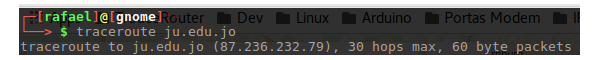
\includegraphics[scale=0.65]{./rota-1.png}
	 		\caption{Inicio de sondagem com um hospedeiro alvo.}
	 		\label{rota-1}
	 	\end{figure}
 	
 	\item
 	Na Figura \ref{rota-2} os três pacotes são enviados para o roteador de borda(roteador que tem conexão com a WAN) com endereço 192.168.1.1, cituado na cidade de Coxim, e são respondidos em ordem pelo mesmo com os tempos de RTT de 0.756 ms, 0.957 ms e 1.129 ms.
 	\begin{figure}[H]
 		\centering
 		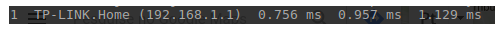
\includegraphics[scale=0.7]{./rota-2.png}
 		\caption{Pacotes são respondidos pelo roteador de borda.}
 		\label{rota-2}
 	\end{figure}
 	
 	\item
 	Na Figura \ref{rota-3} os pacotes encaminhados da borda da rede, chegam para o provedor de Internet nacional, na cidade Brasilia, recebe o os pacotes com TTL zerado, forçando o envio de mensagens ICMP de volta para a máquina originadora da requisição com tempos de RTT de 27.885 ms, 29.145 ms e 32.545 ms.
 	
 	\begin{figure}[H]
 		\centering
 		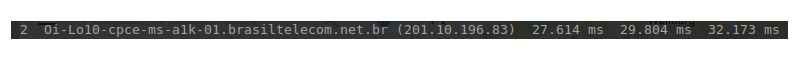
\includegraphics[scale=0.56]{./rota-3.png}
 		\caption{Pacotes são respondidos pelo provedor de Internet nacional, na cidade de Brasília no Brasil.}
 		\label{rota-3}
 	\end{figure}
 
	 \item Na Figura \ref{rota-4}, o endereço do roteador do provedor nacional 200.199.193.135, também na cidade de Brasília, recebe os pacotes com TTL zerado, forçando o envio de mensagens ICMP de volta para máquina originadora da requisição com tempos de RTT de 37.990 ms, 37.994 ms, 41.575 ms. 
	 
	 \begin{figure}[H]
	 	\centering
	 	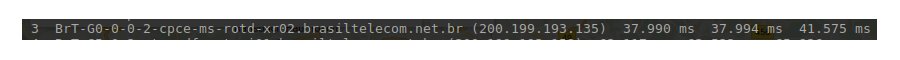
\includegraphics[scale=0.54]{./rota-4.png}
	 	\caption{Pacotes sendo comutados pelos roteadores do provedor nacional, na cidade de Brasília no Brasil.}
	 	\label{rota-4}
	 \end{figure}
 
	\item
	 Na Figura \ref{rota-5}, o endereço do roteador do provedor nacional 200.199.193.159, também na cidade de  Brasília, recebe os pacotes com TTL zerado, forçando o envio de mensagens ICMP de volta para a máquina originadora da requisição com tempos de RTT de 62.117 ms, 63.523 ms, 65.936 ms. 
	
	\begin{figure}[H]
		\centering
		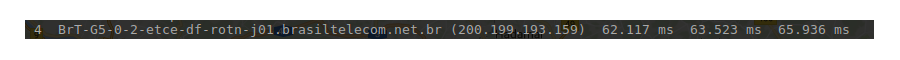
\includegraphics[scale=0.54]{./rota-5.png}
		\caption{Pacotes sendo comutados pelos roteadores do provedor nacional.}
		\label{rota-5}
	\end{figure}
		\item 
		
		Figura \ref{rota-vazia}, o traceroute não consegui resolver as rotas, nos três pacotes enviados, foram respondido mensagens ICMP de tipo 3 (citado na secção \ref{sec:ICMP} ), sendo assim na próxima sondagem ele tentará uma outra rota se disponível.
		
		\begin{figure}[H]
			\centering
			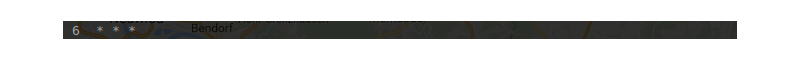
\includegraphics[width=17cm,height=1.3cm]{./rota-vazia.png}
			\caption{Pacotes perdidos.}
			\label{rota-vazia}
		\end{figure}
	
		\item 
		Figura \ref{rota-6}, nessa parte dois pacotes são encaminahdos para o roteador de endereço 177.2.192.100, esse roteador e nacional se encontra na cidade de  Brasília, o mesmo visualiza o TTL zerado, dos pacotes e retorna mensagens ICMP para a máquina originadora da requisição com tempo de RTT de 68.123 ms e 73.770 ms, e um pacote é encaminhado direto para o roteador do servidor Carrier-Grade NAT RFC6598 de endereço 100.120.64.14, que por sua vez, visualiza o TTL zerado retornando uma mensagem ICMP para o máquina originadora da requisição, o RTT desse roteador é de 72.279 ms.
	
	\begin{figure}[H]
		\centering
		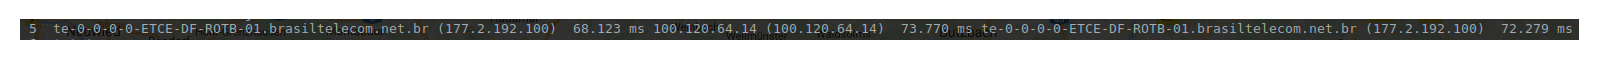
\includegraphics[width=17cm,height=1.3cm]{./rota-6.png}
		\caption{Pacotes sendo comutados pelos roteadores do provedor nacional e provedor de compartilhamento IPv4 Carrier-Grade NAT RFC6598 }
		\label{rota-6}
	\end{figure}

		\item Na Figura \ref{rota-7}, os pacotes são comutados até o um provedor Carrier-Grade NAT RFC6598, com endereço de ip 100.122.17.130 o pacote encaminhado para esse endereço teve um tempo de RTT de 200.617 ms, já o outro pacote foi encaminhado para o mesmo servidor porém com o ip  100.122.17.148 teve um tempo de RTT de 179.446 ms.  
	
	\begin{figure}[H]
		\centering
		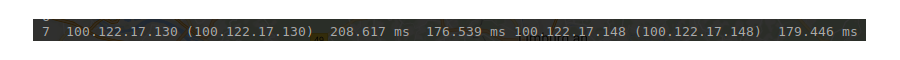
\includegraphics[width=17cm,height=1.3cm]{./rota-7.png}
		\caption{Pacotes sendo comutados pelo servidor Internacional compartilhado IPv4 Carrier-Grade NAT RFC6598.}
		\label{rota-7}
	\end{figure}
	 	
	 	\item Na Figura \ref{rota-8}, assim como na Figura \ref{rota-7} os pacotes são enviados até o enlace de um conjunto de roteadores conhecido como Carrier-Grade NAT RFC6598, que é uma abordagem para o design da rede IPv4 em que os sites finais, em particular as redes residenciais, são configurados com endereços de rede privada que são convertidos para endereços IPv4 públicos por Dispositivos de rede de endereço de rede da middlebox incorporados na rede do operador de rede, permitindo o compartilhamento de pequenos pools de endereços públicos entre vários sites finais. Isso altera a função NAT ea sua configuração das instalações do cliente para a rede do provedor de serviços da Internet, por isso que a sonda do Traceroute encontra alguns endereços IPs vinculado a esse provedor \cite{rfcc}.
	 	
	 	O endereço de ip 100.122.17.149 com tempo de RTT de 191.133 ms, no endereço ip 100.122.17.171 com tempo de RTT de 180.897 e no endereço ip 100.122.17.167 com tempo de RTT de 171.525 ms.
	 	
	 	\begin{figure}[H]
	 		\centering
	 		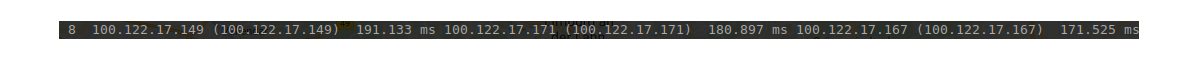
\includegraphics[width=17cm,height=1.5cm]{./rota-8.png}
	 		\caption{Pacotes sendo comutados pelos servidores Internacionais compartilhados Carrier-Grade NAT RFC6598.}
	 		\label{rota-8}
	 	\end{figure}
	 	\item Na Figura \ref{rota-9}, os pacotes foram encaminhados para o endereço 173.205.51.93 do provedor Internacional Tinet GmbH na cidade de New York nos United States, com tempos de RTT de 197.991 ms, 202.254 ms e 202.207 ms.
	 	
	 	\begin{figure}[H]
	 		\centering
	 		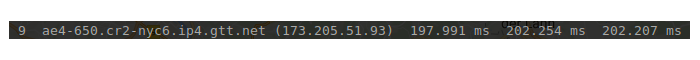
\includegraphics[width=17cm,height=1.5cm]{./rota-9.png}
	 		\caption{Pacotes sendo cumutados até provedor Internacional Tinet GmbH na cidade de New York nos United States.}
	 		\label{rota-9}
	 	\end{figure}
 	
 	 	\item Na Figura \ref{rota-10}, os pacotes foram encaminhados para o endereço ip 141.136.105.222, do provedor GTT Communications Inc, localizado na cidade de Frankfurt Am Main, na Germany, com tempos de RTT de 294.974 ms, 295.028 ms e 297.926 ms..
	 	
	 	\begin{figure}[H]
	 		\centering
	 		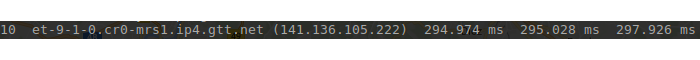
\includegraphics[width=17cm,height=1.5cm]{./rota-10.png}
	 		\caption{Pacotes sendo cumutados até provedor Internacional, GTT Communications Inc, na cidade de Frankfurt Am Main, na Germany.}
	
	 		\label{rota-10}
	 	\end{figure}
 	
	 	 \item Na Figura \ref{rota-11}, os pacotes foram encaminhados para o endereço ip 46.33.83.18, do provedor GTT Communications Inc, localizado na cidade de Isenburg, na Germany, com tempos de RTT de 334.051 ms, 336.230 ms e 339.446 ms.
	 	
	 	\begin{figure}[H]
	 		\centering
	 		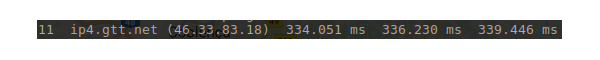
\includegraphics[width=17cm,height=1.5cm]{./rota-11.png}
	 		\caption{Pacotes sendo cumutados até provedor Internacional, GTT Communications Inc, na cidade de Isenburg, na Germany.}
	 		\label{rota-11}
	 	\end{figure}
 	
	 	 \item Na Figura \ref{rota-12}, os pacotes foram encaminhados para o endereço ip 213.139.41.2, do provedor Jordan Telecommunications Company, localizado na cidade de Amman, na Jordan, com RTT de 299.414 ms, 300.090 ms e 299.396 ms.
	 	
	 	\begin{figure}[H]
	 		\centering
	 		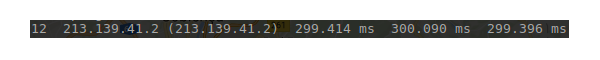
\includegraphics[width=17cm,height=1.5cm]{./rota-12.png}
	 		\caption{Pacotes sendo cumutados até provedor Internacional, Jordan Telecommunications Company, na cidade de Amman, na Jordan.}
	 		\label{rota-12}
	 	\end{figure}
 	
	 	 \item Na Figura \ref{rota-13}, os pacotes foram encaminhados para o endereço ip 213.139.32.206, do provedor Jordan Telecommunications Company, também localizado na cidade de Amman, na Jordan, com RTT de 310.995 ms, 311.614 ms e 311.892 ms.
	 	
	 	\begin{figure}[H]
	 		\centering
	 		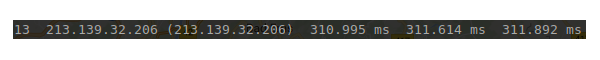
\includegraphics[width=17cm,height=1.5cm]{./rota-13.png}
	 		\caption{Pacotes sendo cumutados até provedor Internacional, Jordan Telecommunications Company, na cidade de Amman, na Jordan.}
	 		\label{rota-13}
	 	\end{figure}
 \end{enumerate}

	O último salto realizados nos roteadores até a maquina hospedeira foi o de numero 13, mostrado na Figura \ref{rota-13}, mostrando assim o funcionamento do traceroute, os outros 17 saltos restantes são descartados pelo traceroute (como citado na secção \ref{sec:funcioanemnto}), já que não existe mais roteadores acessíveis disponiveis para dar continuidade a sondagem, Figura \ref{traceroute}.
	
\begin{figure}[H]
	\centering
	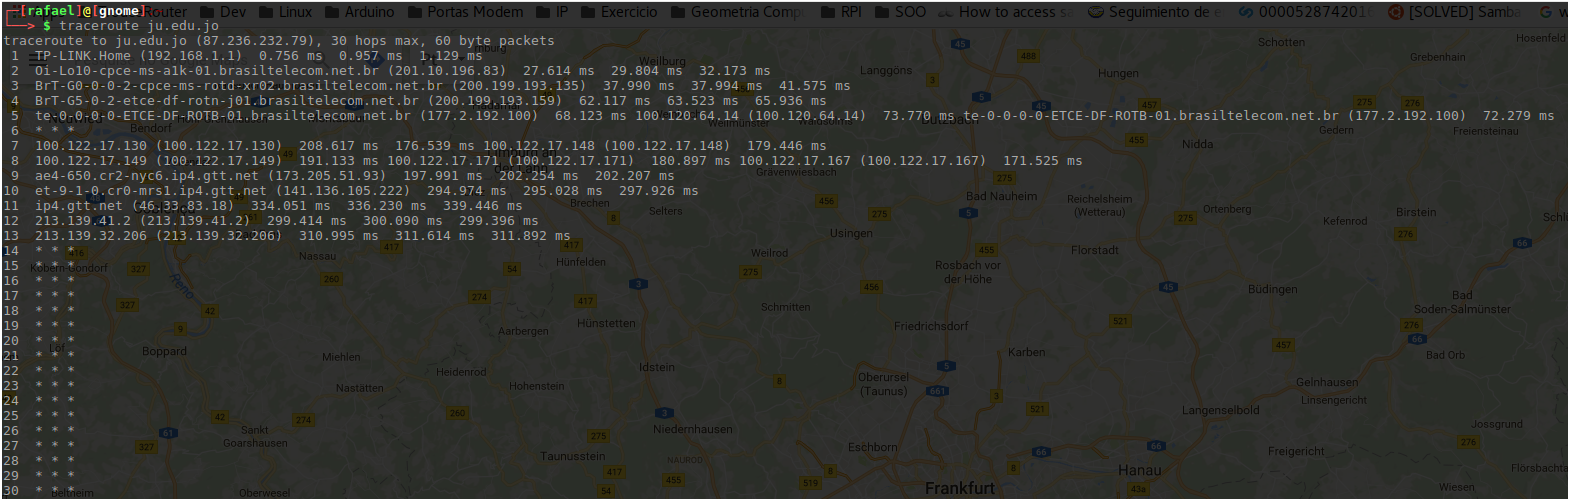
\includegraphics[width=15cm,height=8cm]{./trauceroute-1.png}
	\caption{Resultado final da sondagem utilizando o Traceroute.}
	\label{traceroute}
\end{figure}
	 

\subsubsection{Mapeamento utilizando Google Earth }
	Com base nos endereços IPs fornecido pelo Traceroute, foi descoberto as coordenadas geográficas dos IPs, pelo o site www.localizaip.com.br (contendo variaç\~oes nas coordenadas), com essas coordenadas foi mapeado a apenas as rota Internacionais que os pacotes traferam na Internet (a coordenada que foi apresentada pelo localizaip.com referente aos IPs dos roteadores Carrier-Grade NAT RFC6598 apontaram para as coordenadas Latitude=0.0 e Longitude=0.0, sendo assim a posição geográfica não corresponde com a posição real), utilizando o Google Earth para fazer as marcações no Mapa Gobal Figura \ref{google-earth}.
\begin{figure}[H]
	\centering
	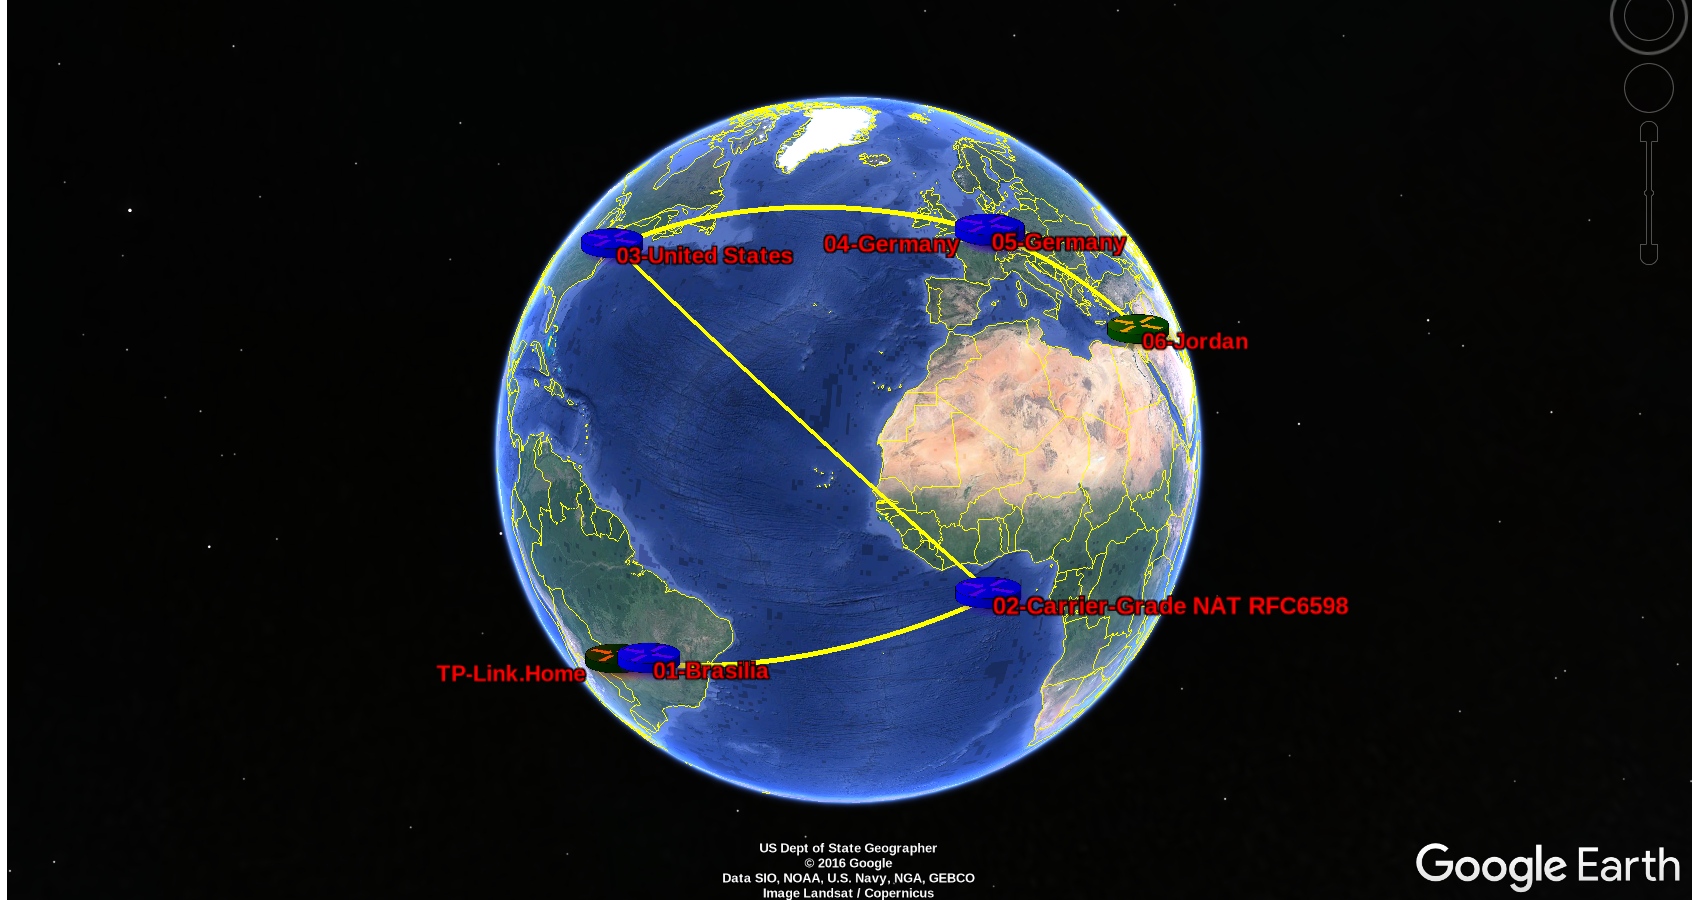
\includegraphics[width=15cm,height=11cm]{./google-earh.png}
	\caption{Mapeamento das rotas Internacioais, até a Jordania apartir dos endereços de IPs fornecido pelo Traceroute.}
	\label{google-earth}
\end{figure}

% ---
% Finaliza a parte no bookmark do PDF, para que se inicie o bookmark na raiz
% ---
\bookmarksetup{startatroot}% 
% ---

% ---
% Conclusão\part{title}
% ---
\section{Considerações finais}
  Com a ferramente Traceroute podemos análisar o percurso dos pacotes até seu destino, podendo assim observar por onde nossos pacotes estão passando (sendo cumutados pela rede), melhorando a apuração de possíveis problemas (firewalls, congestionamentos na rede, entre outros), entre a máquina remetente e a máquina destinatária, sendo possível, a análise por meio de respostas ICMP (citado na  \ref{sec:ICMP}) provocadas propositalmente pelos campos TTL zerados (citado na secção \ref{sec:IPv4}) ou por portas altas não acessível, saltando pelos roteadores do núcleo da rede um-a-um até a máquina hospedeira.
  

\bibliographystyle{abntex2-alf}
\bibliography{abntex2-modelo-references}



\end{document}
